%设置页面边距(word标准页面)
\documentclass[a4paper]{article}
\usepackage{geometry}
\geometry{a4paper,left=2.7cm,right=2.7cm,top=2.54cm,bottom=2.54cm}
 
%导入ctex包
\usepackage[UTF8,heading=true]{ctex}
 
%设置摘要格式
\usepackage{abstract}
\setlength{\abstitleskip}{0em}
\setlength{\absleftindent}{0pt}
\setlength{\absrightindent}{0pt}
\setlength{\absparsep}{0em}
\renewcommand{\abstractname}{\textbf{\zihao{4}{摘要}}}
\renewcommand{\abstracttextfont}{\zihao{-4}} %设置摘要正文字号
 
%设置页眉和页脚,只显示页脚居中页码
\usepackage{fancyhdr}
\pagestyle{plain}
 
%调用数学公式包
\usepackage{amssymb}
\usepackage{amsmath}
 
%调用浮动包
\usepackage{float}
\usepackage{subfig}
\captionsetup[figure]{labelsep=space} %去除图标题的冒号
\captionsetup[table]{labelsep=space} %去除表格标题的冒号
%设置标题格式
\ctexset {
	%设置一级标题的格式
	section = {
		name={,、},
		number=\chinese{section}, %设置中文版的标题
		aftername=,
	},
	%设置三级标题的格式
	subsubsection = {
		format += \zihao{-4} % 设置三级标题的字号
	}
}
 
%使得英文字体都为Time NewTown
\usepackage{times}
 
%图片包导入
\usepackage{graphicx}
\graphicspath{{images/}} %图片在当前目录下的images目录
 
%参考文献包引入
\usepackage{cite}
\usepackage[numbers,sort&compress]{natbib}
 
%代码格式
\usepackage{listings}
\usepackage{graphicx}%写入python代码
\usepackage{pythonhighlight}%python代码高亮显示
\lstset{
	numbers=left, %设置行号位置
	numberstyle=\small, %设置行号大小
	keywordstyle=\color{blue}, %设置关键字颜色
	commentstyle=\color[cmyk]{1,0,1,0}, %设置注释颜色
	escapeinside=``, %逃逸字符(1左面的键),用于显示中文
	breaklines, %自动折行
	extendedchars=false, %解决代码跨页时,章节标题,页眉等汉字不显示的问题
	xleftmargin=-1em,xrightmargin=-1em, aboveskip=1em, %设置边距
	tabsize=4, %设置tab空格数
	showspaces=false %不显示空格
}

\renewcommand{\refname}{}
 
%item包
\usepackage{enumitem}

%跨页长三线表
\usepackage{longtable}
 
%表格加粗
\usepackage{booktabs}
 
%设置表格间距
\usepackage{caption}

%独立设置表格水平线粗细
\usepackage{makecell} 
 
%允许表格长跨页
\usepackage{longtable}
 
%伪代码用到的宏包
\usepackage{algorithmic}
\usepackage{algorithm}
 
%正文区
\title{\textbf{基于连续性原理的相位展开法的InSAR高程恢复方法}}
\date{} %不显示日期
 
%文档
\begin{document}
	\maketitle
	\vspace{-6em} %设置摘要与标题的间距
	\zihao{-4} %设置正文字号
	%摘要部分
	\begin{abstract}

		干涉合成孔径雷达(Interferometric Synthetic Aperture Radar,InSAR)是一种先进的遥感技术,用于精确测量和监测地表形变。近年来随着自然灾害频发和城市化进程加快,对地表形变的监测需求日益增加,InSAR技术的应用前景愈发广阔。\par
		本文主要针对于高程恢复中的相位解缠问题进行讨论,先后建立了基于相位展开的连续性原理方法和LSTM神经网络的两种数学模型,并取得了良好的解缠效果,高程恢复基本实现。在此过程中,我们还讨论了计算效率和规模的优化问题,采用尽可能少的数据达到精度要求。\par
		针对问题一,我们首先对原始数据进行了数据清洗、打表、可视化等的数据处理操作,对原始数据规律进行了初步的分析,观察、总结出初步规律,提取出问题的关键在于相位解缠和数据选择。接着,我们根据已有的公开文献,寻求相位解缠方法,探讨并实验了其中几种模型的可行性,最终形成了数学方法和机器学习方法各一种,接着利用python进行了编程实现,成功完成了相位解缠。接着,我们对双缝干涉原理进行分析,在排除误差较大的数据后,通过对采样次数和单次采样精度两方面的综合考量,选择出了第2和第5两组数据,并利用推广的3维相位展开法对两组数据进行融合,利用python进行了编程实现,得到的高程恢复效果非常好,精度符合预期要求。\par
		针对问题二,我们由问题一的结果发现确实如题干所述,选取更多的数据可以减少误差对高程估计的影响,在数据清洗过后考虑到对所有数据的二项式组合量级不是非常大,故遍历所有组合恢复出的高程值,对这些数据进行方差与梯度及分辨率分析作为精度评估,以选取数据的数组个数作为复杂度评估,引入一个分数奖惩体系,综合以上方面的分数选出精度被保证的前提下的最优数组选取策略。在我们的模型下,经过综合评估,发现综合选取两组数据时分数整体最优,并且在两组数据的选取方式下,发现选择第2和第5组数据的分数最优。\par
		针对问题三,\\
		%关键词(上文最后一段要用“\\”换行)
		\newline
		\noindent{\textbf{关键词:} \textbf{InSAR}\quad  \textbf{相位解缠}\quad  \textbf{相位展开法}\quad  \textbf{LSTM}\quad  \textbf{综合评价方法}\quad} 
	\end{abstract}
	
	\clearpage %换页
	
	%正文部分
	%Part one
	\section{问题背景与重述}
	\subsection{问题背景}

	近年来,干涉合成孔径雷达(Interferometric Synthetic Aperture Radar, InSAR)遥感理论与技术处于快速发展的态势,InSAR信息的提取主要依赖于干涉相位和搭载SAR传感器的平台位置与姿态数据,如基线参数的处理与分析,可广泛应用于地形测量,特别是数字高程模型(digital elevation model, DEM)的生成。InSAR目前已经成为一种重要的对地观测遥感技术手段,被广泛应用在环境监测、灾害监测、山体滑坡等领域,因此具有重要的研究意义。\par
	在实际求解过程中会遇到如下两个难题:其一,相位缠绕的问题,即测得的相位与真实的相位之间相差的整倍数,这个现象也被称为相位模糊,相位缠绕常发生于山地、城市等地形复杂的区域或断崖、裂谷等地形变化较大的地方。其二,由于测量的过程中误差不可避免,故会导致测得的相位带有误差,这给高程的恢复带来了极大的困难,同时由于高程图像本身含有多个像素点,信息量已足够庞大,因此一味增多观测数据来减小误差的方法并不可取,选择尽可能少的观测数据达到较高的恢复精度也是研究一大重点内容。
	
	%\begin{figure}[H]
	%	\centering %图片居中
	%	\captionsetup{skip=4pt} % 设置标题与表格的间距为4pt
	%	\includegraphics[width=10cm]{图片文件名} %width设置图片大小
	%	\caption{商超蔬菜示意图\label{商超蔬菜示意图}} %设置图片的标题及引用标签
	%\end{figure}
	
	\subsection{问题重述}
	
	基于上述背景,我们需要建立数学模型解决以下问题:

	\begin{enumerate}[itemindent=0.5cm]
		\item 如何设计一数学模型对原数据进行高程恢复
		\item 如何在达到预期精度的前提下,使用尽量少的数据(减小计算规模)
		\item 分析误差对所建模型的影响
	\end{enumerate}
	
	%Part Two
	\section{问题分析}
	\subsection{问题一的分析}

	本问题主要探讨如何进行InSAR高程恢复。为了达到这一目的,我们从相位解缠和数据选择两方面进行考虑。\par
	一、相位解缠:相位缠绕问题起因于地形高度的变化超过了一个波程长度(即相位变化超过了$ 2\pi $),但仪器无法记录这种周期性变化(只记录一个周期内的绝对相位),因此需要找出缠绕前的相位来恢复真实高度。由于真实相位与高程之间的函数关系式过于复杂,赛题基于从易入题的角度考虑,给出了简化的模型:\par
	\begin{equation}
		h = -\frac{1}{k_z} \cdot \varphi
	\end{equation}
	其中,$ k_z $为事先设定的值,范围在$ [0,1] $之间;$ \varphi = \theta + 2n\pi $为真实的相位;$ \theta $为测量相位,范围在$ [0,2\pi) $之间。\par
	由此出发,我们形成了以下初步分析与建模规划:\par
	1.原始数据分析:根据给出的原始数据,不加处理地绘制出5组数据的“测量高程色度图”,观察高程的分布规律,由此给出适当猜测(详见第三部分“模型假设”)。\par
	2.寻求相位解缠方法:相位解缠主要包括数学方法和机器学习方法,需要分别使用两类方法进行相位解缠,并进行对比、印证,从而考察方法的优劣度和结果的准确性。\par
	二、数据选择:多次测量信息综合可以大大减小实验误差,提升测量精度,但InSAR高程观测数据规模通常很大,在算力有限的前提下无法采用全部观测数据进行高程恢复,因此需要在达到精度要求的前提下,选出的高精度观测数据(主成分)尽量少。赛题规定从5组数据中选取2组进行高程恢复,并要求精度在1m以内。\par
	由此出发,我们形成了以下初步分析与建模规划:\par
	1.将数据选择的依据分解为精度和复杂度,其中,复杂度与数据组数成正相关关系,且题目已限制为2组数据,可暂不考虑。\par
	2.找寻合适的精度量化指标,并讨论它们在反应数据优良性方面所起到的作用的大小,最终给出数据选择和综合后的高程结果。\par

	\subsection{问题二的分析}

	本问题紧承上一问的第二小问对于数据选择的讨论,提出了在达到精度要求的前提下,尽可能减小计算复杂度或所选取的数组个数最少。为了达到这一目的,我们利用基于奖惩体系的综合评价方法进行分析。\par
	评价哪一种组合方案最优应该同时考虑方案的精度和复杂度,而要综合这两个指标考虑问题,需要先建立指标体系。我们试图建立以不同数据组合为方案,总精度和复杂度(组数)为评价指标的综合评价体系,如下表1所示:\par
	
	\begin{table}[H] %[h]表示在此处添加浮动体,默认为tbf,即页面顶部、底部和空白处添加
		\captionsetup{skip=4pt} % 设置标题与表格的间距为4pt
		\centering
		\caption{总精度和复杂度量化指标体系}
		\setlength{\arrayrulewidth}{1pt} % 设置表格线条宽度为1pt
		\begin{tabular}{c|cc} %c表示居中,l表示左对齐,r表示右对齐,中间添加“|”表示竖线
			\Xhline{1.5pt}
			\makebox[0.2\textwidth][c]{方案} & \makebox[0.5\textwidth][c]{总精度} & \makebox[0.2\textwidth][c]{复杂度(组数)} \\ 
			\hline
			2 + 3 & xxx & 2 \\
			2 + 4 & xxx & 2 \\
			2 + 5 & xxx & 2 \\
			3 + 4 & xxx & 2 \\
			3 + 5 & xxx & 2 \\
			4 + 5 & xxx & 2 \\
			2 + 3 + 4 & xxx & 3 \\
			2 + 3 + 5 & xxx & 3 \\
			2 + 4 + 5 & xxx & 3 \\
			3 + 4 + 5 & xxx & 3 \\
			2 + 3 + 4 + 5 & xxx & 4 \\
			\hline
			共 11 种 & -- & -- \\
			\Xhline{1.5pt}
		\end{tabular}
		% \hline是横线,采用\makebox设置列宽
	\end{table}

	我们采用**来量化精度,用参与拟合的数据组数量化复杂度。这些指标都是极小型指标,需要转化为极大型指标,并继续经过标准化处理,计算赋予权重,最终综合评估每个方案的优劣。\par
	首先采用极差变换法将数值型指标转化为极大型指标。将一致化处理后的指标进行标准化处理,得到评价矩阵。之后使用变异系数法计算权重向量,得到权重矩阵。最后根据权重矩阵和评价矩阵,计算每个方案的综合评价值向量。得到方案排名,从中选出最优方案。\par

	\subsection{问题三的分析}

	在该过程中,误差来源主要包括相位缠然现象产生的系统误差和测量过程中的随机误差两类。系统误差只能通过改进测量原理的方法消除。随机误差可以通过多次测量取平均或提取主成分等方法来减弱,但不能完全消除。基于这两种误差来源,我们对该问题中误差对相位高程恢复的影响进行分析,并得出结论。\par
	
	%Part Three
	\section{模型假设}
	%假设的列表
	\begin{enumerate} 
		\item 假设真实高程为连续曲面,即相邻像素点之间的高程差为一个相对于精度而言小量。
		\item 假设图样为理想的干涉条纹图,即条纹图满足Nyquist采样定理。任意两个采样点之间的非截断相位差的值在$ -\pi $到$ \pi $之间。
		\item 缠绕相位信息中没有噪声。
	\end{enumerate}
	
	%Part Four
	\section{符号说明}
	%浮动体表格,使用table实现
	\begin{table}[H] %[h]表示在此处添加浮动体,默认为tbf,即页面顶部、底部和空白处添加
		\captionsetup{skip=4pt} % 设置标题与表格的间距为4pt
		\centering
		\setlength{\arrayrulewidth}{1.5pt} % 设置表格线条宽度为1pt
		\begin{tabular}{cc} %c表示居中,l表示左对齐,r表示右对齐,中间添加“|”表示竖线
			\hline
			\makebox[0.15\textwidth][c]{符号} & \makebox[0.79\textwidth][c]{说明}  \\ 
			\toprule
			r & Spearman系数  \\
			 &   \\
			\hline
		\end{tabular}
		% \hline是横线,采用\makebox设置列宽
	\end{table}
	
	
	%Part Five
	\section{模型的建立与求解}
	\subsection{InSAR地形高程测量原理}

	为了更好地进行建模,需要先理解InSAR的工作原理。合成孔径雷达干涉测量(InSAR)是一种用于获取目标区域高程信息及其变化的技术。其基本原理是提取两幅同一地区的 SAR(合成孔径雷达)影像数据的相位信息。\par
	InSAR 的工作方式有两种主要模式:\par
	1. 单轨道双天线模式:在同一飞行平台上安装了两副天线,分别记为 S1 和 S2。这两副天线都发射和接收信号,因此一次飞行就可以获得对同一地区的重复干涉数据。这种模式下,相位信息是通过两副天线同时获取的,因此称为双天线模式。\par
	2. 重复轨道单天线模式:在不同的时间和不同的轨道上获取了两幅影像。在这种模式下,同一地区的两次观测是在相邻轨道上,具有一定的时间间隔。每次观测中只有一副天线(通常是在单一飞行平台上的同一 SAR 系统)。因此,这种模式下称为单天线模式。\par
	不论是哪种模式,目标和两副天线之间的距离不同,因此目标反射回来的回波信号由于距离的不同而产生时间差。这种时间差在相位上就表现为相位差。通过对两幅影像的相位信息进行比较,可以得到相位差影像。结合相应的 SAR 系统的轨道参数和传感器参数,就可以推导出目标的高程信息。
	
	\begin{figure}[H] %[h]表示图片放在当前位置(here),H表示强制紧接在上文的后面
		\centering %图片居中
		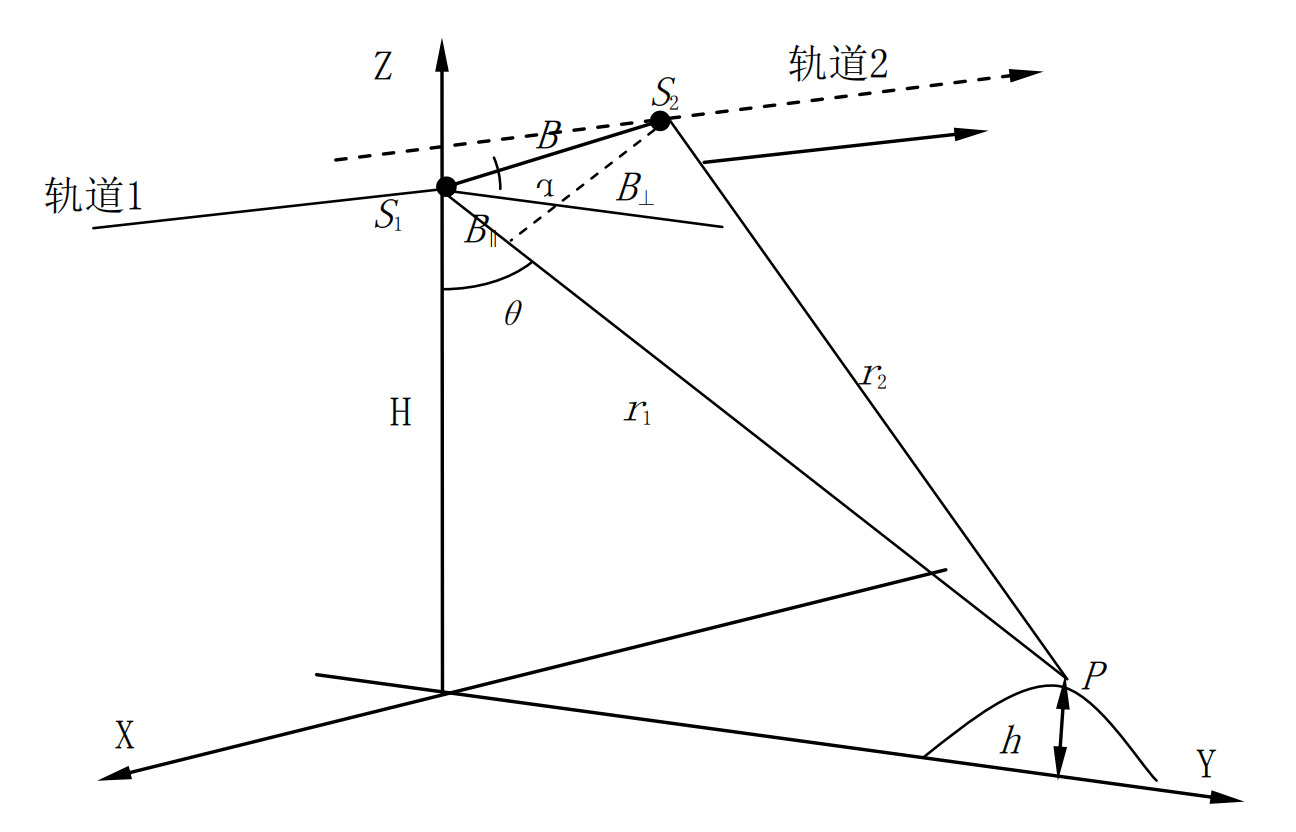
\includegraphics[width=0.8\textwidth]{insar_priciple.png} %图片文件名和宽度设置
		\caption{合成孔径雷达干涉测量测高原理示意图}
		\label{fig:insar_principle} %用于引用的标签
	\end{figure}
	
	\subsection{问题一的模型建立及求解}

	通过对InSAR原理的分析可知,利用相位差和相位周期性变化的信息进行相位解缠是一种非常可行的策略。目前已有的基于相位差的相位解缠数学方法很多,在如今人工智能迅速发展的背景下,基于机器学习的相位解缠方法也如雨后春笋般层出不穷。数学方法主要有结合快速傅里叶变换(FFT)或二维离散反余弦变换(DCT)等的最小二乘法、Goldstein路径积分算法等,机器学习方法主要有LSTM自动编码器、PGE-PCA网络算法、R2AU-Net方法等。综合评估各种方法的实现难度和预测效果,我们设计了一种数学方法进行相位解缠,并使用在一篇文献中得到的LSTM自动编码器模型进行了对照检验。

	\subsubsection{数据预处理}

	因为python在二维数据处理和科学计算方面有着优秀性质和众多实用的模版库,因此我们选定编程语言为python,并利用python对原始数据进行了如下的预处理(代码见附录7.1):\par
	1.存储$ k $值的数据集中,第一行$ k $值的尾部存在$ .x $的列编号,需要使用python中的字符串操作进行删除。\par
	2.将原.xlsx格式转换为.csv格式,有利于python的快速读取。

	\subsubsection{数学方法}

	由原始$ k $值和观测相位$ \theta $直接计算得到的高程色度图如下(代码见附录7.2):\par
	
	\begin{figure}[H]
		\centering
		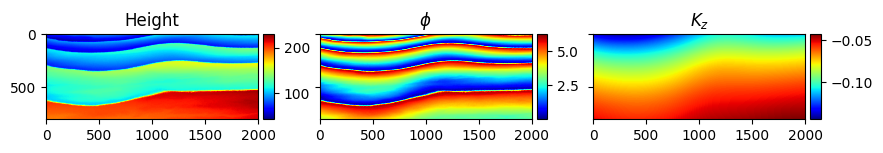
\includegraphics[width=1.01\textwidth]{images/raw/raw_1.png}
		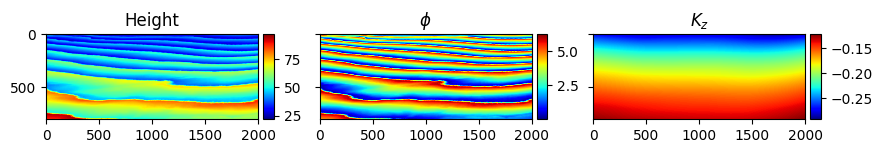
\includegraphics[width=1.01\textwidth]{images/raw/raw_2.png}
		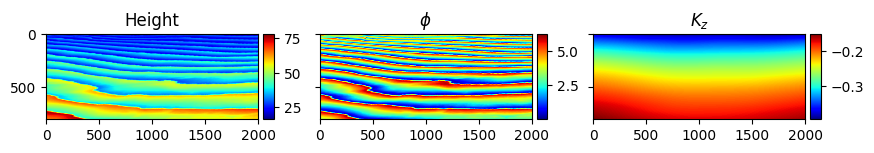
\includegraphics[width=1\textwidth]{images/raw/raw_3.png}
		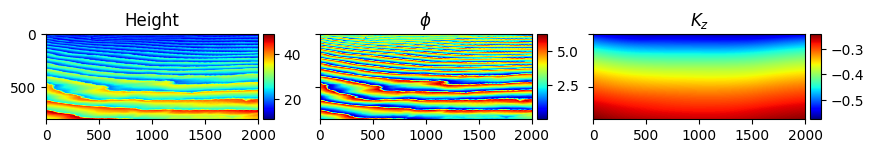
\includegraphics[width=1\textwidth]{images/raw/raw_4.png}
		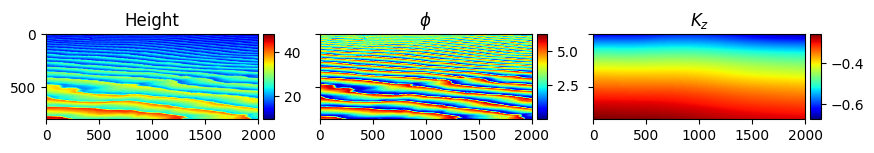
\includegraphics[width=1\textwidth]{images/raw/raw_5.png}
		
		\caption{原始数据高程色度图绘制}
		\label{fig:raw_1}
	\end{figure}

	从图2可以看出,高程和观测相位呈现出一种明显的波纹状周期性变化规律。但第1组数据的干涉条纹宽度过大,相位的相干性较低,与其余四组数据有明显的差值,对高程恢复没有直接帮助,因此可以暂时舍去,对余下的2到5共4组数据进行如下建模:\par
	由光(电磁波)的干涉理论可知:当两束或多束相干光相遇时,它们会叠加在一起。根据光波的相对相位差不同,有如下两种强叠加情形:\par
	1.当两束光的相位相同或相差为偶数倍的时候,它们的波峰和波峰、波谷和波谷相互叠加,形成更亮的条纹,这种现象称为相长干涉(constructive interference)。\par
	2.当两束光的相位差为奇数倍的时候,它们的波峰和波谷相互抵消,形成更暗的条纹,这种现象称为相消干涉(destructive interference)。\par
	雷达波的干涉原理与双缝干涉同根同源,根据上述原理可以得到相位解缠的核心原理:在InSAR单轨道双天线模式的一次测量过程中,两天线发出的波相同,具有相干性;飞行载体的轨道高度尺度远大于两天线间距的尺度,满足杨氏双缝干涉实验的条件,从而可以通过双缝干涉条纹叠加原理得到InSAR相位解缠的实现方法和精度评估标准。\par

	双缝干涉条纹宽度和双缝间距的关系由以下公式给出:\par
	\begin{equation}
		\Delta x = L \cdot \frac{\lambda}{d}
	\end{equation}
	其中:\par
	$ \Delta x $表示条纹宽度,对应于解缠前高程色度图的条纹宽度\par
	$ L $表示光屏到双缝的距离,对应于飞行载体的轨道高度\par
	$ d $表示双缝宽度,对应于两天线之间的距离\par
	$ \lambda $表示光的波长,对应于两天线发出的相干波波长\\

	在InSAR单轨道双天线模式的一次测量过程中,由于地球为近似椭球面以及地形突变或复杂等的干扰因素,双天线会接收到若干近似等间距平行条纹的相位信息。每个条纹都分别存储了测量区域的全部信息,因为一次测量中存在周期性变化,从而元区域大小的图像上会有若干这样的条纹同向平行排列,并且随着$ n $的增大,干涉波的角度增大,在光学上反映为光强减弱,条纹变暗;在InSAR相位图上反映为相位变化越模糊,信息精度越低,因此在相位数据关于中心条纹对称的条件下,越靠近中心的相位数据越精确,越往两侧的相位数据越失真。此外,因为相消干涉的影响,两相邻条纹的边界处的相位信息的准确度将会大幅度降低。\par
	对于单组数据的精度有:条纹数目越多,说明采样次数越多,信息量越大,对总精度会产生有利影响,反之亦然;单个条纹宽度越宽,说明一次采样精度越高,对总精度会产生有利影响,反之亦然。同时,因为存储容器的容量限制,在达到高采样次数的条件下,单次采样精度必然降低;反之低采样次数会获得更好的单次采样精度。我们可以用不确定关系描述二者的关系:\par
	\begin{equation}
		N \cdot \sigma \leq k
	\end{equation}	
	其中,$ N $为采样次数,$ \sigma $为单次采样精度,$ k $为一个正常数。
	
	\paragraph{基于连续性原理的相位展开法的高程恢复}
	我们采用的数学方法是相位展开法(代码见附录7.3),在双缝干涉模型下,相位数据受到干涉现象周期性的影响从而导致相位纠缠,相位展开的目的就是将这些相位数据的位置复原,转换成具有连续性的形式。\par
	InSAR观测的相位值均在$ [0,2\pi] $的范围内,折叠了$ 2\pi $整数倍扫描周期的信息。基于相位的连续性原理可知,真实相邻相位之间的差应该在$ [-\pi,\pi] $之间,并且满足:\par
	\noindent1.水平方向上:\par\indent
	对于每一列的所有相位,通过计算每个相位与其前一列相位之间的相位差,同时对$ 2\pi $取模运算将该差异归一化到$ [-\pi,\pi] $范围内,并累加到前一列展开相位值中,实现相位在水平方向上的连续排列。数学表达如下:\par
    \begin{subequations}
		\begin{align}
			\Delta \theta_i = \theta[i, 0] - \theta[i-1, 0] \\
			\Delta \theta_{\text{wrapped}} = (\Delta \theta_i + \pi) \mod 2\pi - \pi \\
			\phi[i, 0] = \phi[i-1, 0] + \Delta \theta_{\text{wrapped}}
		\end{align}
	\end{subequations}
	2.垂直方向上:\par
	对于每一行的所有相位,通过计算每个相位与其前一行相位之间的相位差,同时对$ 2\pi $取模运算将该差异归一化到$ [-\pi,\pi] $范围内,并累加到前一行展开相位值中,实现相位在垂直方向上的连续排列。数学表达如下:\par
	\begin{subequations}
		\begin{align}
			\Delta \theta_j = \theta[0, j] - \theta[0, j-1] \\
			\Delta \theta_{\text{wrapped}} = (\Delta \theta_j + \pi) \mod 2\pi - \pi \\
			\phi[0, j] = \phi[0, j-1] + \Delta \theta_{\text{wrapped}}
		\end{align}
	\end{subequations}
	3.其他方向上:\par
	对于矩阵中其他位置的元素,分别计算其与前一行元素及前一列元素的相位差,用与上面同样的方法将这些差异归一化到$ [-\pi,\pi] $范围内,然后分别累加到前一个展开相位值中,实现在其他方向上的连续排列。数学表达如下:\par
	\begin{subequations}
		\begin{align}
			\Delta \theta_{\text{row}} = \theta[i, j] - \theta[i-1, j] \\
			\Delta \theta_{\text{col}} = \theta[i, j] - \theta[i, j-1] \\
			\Delta \theta_{\text{row wrapped}} = (\Delta \theta_{\text{row}} + \pi) \mod 2\pi - \pi \\
			\Delta \theta_{\text{col wrapped}} = (\Delta \theta_{\text{col}} + \pi) \mod 2\pi - \pi \\
			\phi[i, j] = \phi[i-1, j] + \Delta \theta_{\text{row wrapped}} \\
			\phi[i, j] = \phi[i, j-1] + \Delta \theta_{\text{col wrapped}}
		\end{align}
	\end{subequations}\indent
	
	在此问题中,上述操作表现为每个像素点与以其为中心的东、西、南、北、东北、西北、东南、西南方向上的像素点之间的相位差均在$ [-\pi,\pi] $范围内,即实现了全方向上的连续排列。\par
	展开后的相位仍然不在$ [150,300] $的参考范围内,因此需要对相位进行整体调整。此过程采用对n迭代的方法,每次对相位整体增加一个周期($ 2\pi $),直至所有高程值落在限定范围内。由于题目数据的特殊性,迭代后的相位落在规定区间内的n恰好都只有唯一解,这也从一个侧面印证了本方法的正确性(代码见附录7.4)。\par
	图3\footnote{图3的第3列图像上方的数字,第1位代表数据集编号,第2-3位表示迭代n的次数。}为经过2维相位展开法展开后,2到5各组数据的高程色度图像:\par
	
	\begin{figure}[H]
		\centering
		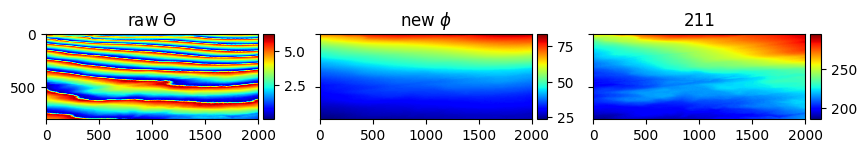
\includegraphics[width=1\textwidth]{images/t1/unwrap2.png}
		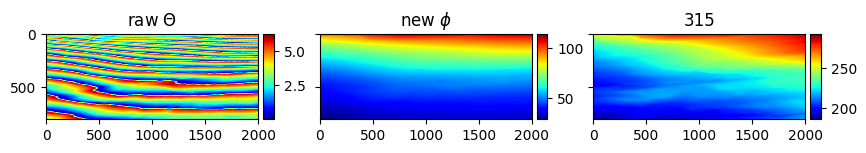
\includegraphics[width=1\textwidth]{images/t1/unwrap3.png}
		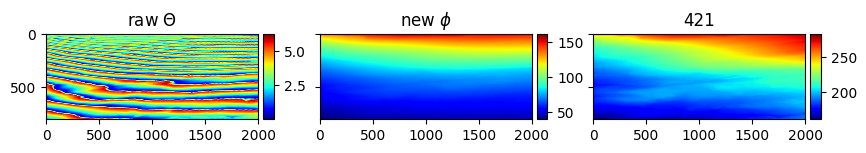
\includegraphics[width=1\textwidth]{images/t1/unwrap4.png}
		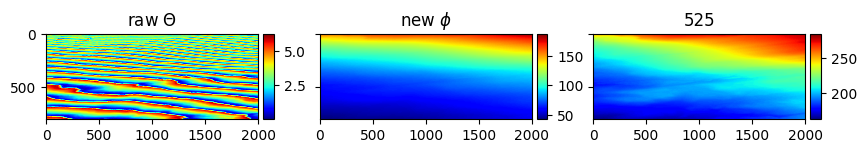
\includegraphics[width=1\textwidth]{images/t1/unwrap5.png}
		
		\caption{解缠后数据高程色度图绘制}
		\label{fig:unwrap}
	\end{figure}

	同时给出高程恢复后各组数据的3D地形实景模拟图,如图4所示:\par

	\begin{figure}[H]
		\centering
		\begin{minipage}[b]{0.4\textwidth}
			\centering
			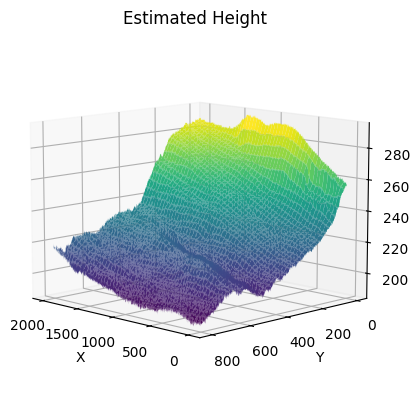
\includegraphics[width=\linewidth]{images/t1/unwrap3d_2.png}
		\end{minipage}
		\hspace{0.05\textwidth}
		\begin{minipage}[b]{0.4\textwidth}
			\centering
			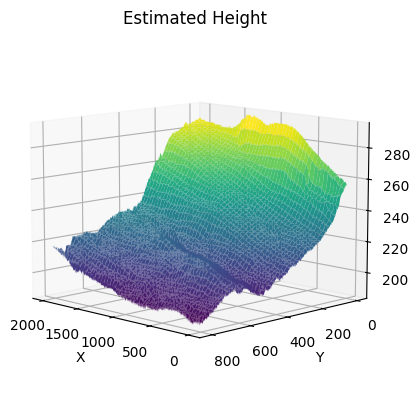
\includegraphics[width=\linewidth]{images/t1/unwrap3d_3.png}
		\end{minipage}

		\begin{minipage}[b]{0.4\textwidth}
			\centering
			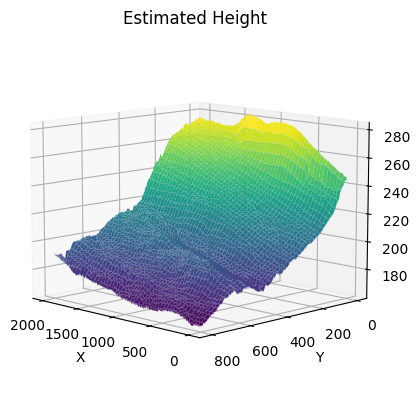
\includegraphics[width=\linewidth]{images/t1/unwrap3d_4.png}
		\end{minipage}
		\hspace{0.05\textwidth}
		\begin{minipage}[b]{0.4\textwidth}
			\centering
			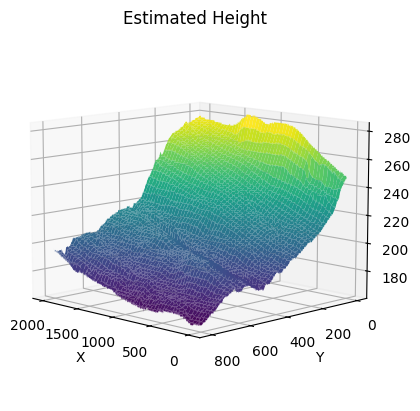
\includegraphics[width=\linewidth]{images/t1/unwrap3d_5.png}
		\end{minipage}

		\caption{高程恢复后的3D地形实景模拟图}
		\label{fig:unwrap3d}
	\end{figure}	

	\paragraph{最佳数据组合}
	精度是本小题中唯一需要考虑的数据选择依据。我们进一步将单组数据的总精度分解为采样次数和单次采样精度两个维度。由二者的不确定性关系可知,解缠后的4组相位编号从小到大依次呈现出采样次数提升,单次采样精度下降的变化趋势。因此,最佳的数据组合应该为第2组和第5组数据,其中第2组数据具有最高的单次采样精度,第5组数据就有最大的采样次数。综合2和5的信息,就可以得到一个在采样次数和单次采样精度两方面都有很高水平的修正相位图。\par
	受到2维相位展开法思路的启发,我们创新性地将其扩展到了3维的情况:将数据组编号设置为第3个维度,以该维度堆叠两个数据集的解缠相位矩阵,构建出一个形状为$ 805\times2001\times2 $的3维矩阵。对该矩阵应用3维相位展开法即可得到两组数据的综合结果。3维相位展开法的数学表达式如下(代码见附录7.7):\par
	\noindent1.在单个解缠相位平面内:\par\indent
	和2维相位展开法的情形类似,每个相位只添加了一个反映其在3维相位矩阵中层次信息的编号,该编号在层中不发生变化,因而解缠算法与2维的情形完全相同,此处不再赘述。\par
	\noindent2.层次间相位融合:\par\indent
	计算当前层与前一层之间的相位差,将该相位差归一化到$ [-\pi,\pi] $范围内,并更新展开后的相位值,由此实现了层次之间的相位信息组合,并且保留了各层的优良性质。数学表达如下:\par
	\begin{subequations}
		\begin{align}
			\Delta_{\text{depth}} = \theta[i,j,k] - \theta[i,j,k-1] \\
			\Delta_{\text{depth, wrapped}} = \left( \Delta_{\text{depth}} + \pi \right) \bmod 2\pi - \pi \\
			\phi[i,j,k] = \phi[i,j,k-1] + \Delta_{\text{depth, wrapped}}
		\end{align}
	\end{subequations}
	
	根据第2和第5组数据,经过2、3维相位展开后所得的融合高程色度图如下图5所示(代码见附录7.8):\par

	\begin{figure}[H]
		\centering
		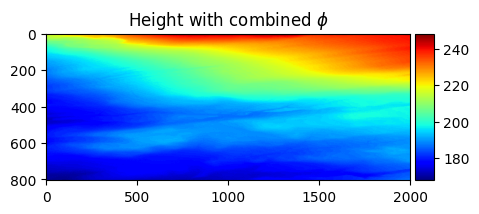
\includegraphics[width=0.6\textwidth]{t1/output_1_2.png}
		\caption{最佳高程恢复色度图}
		\label{fig:best_phi}
	\end{figure}

	同时绘制出最佳高程恢复后的3D地形实景模拟图(如下图6所示):\par

	\begin{figure}[H]
		\centering
		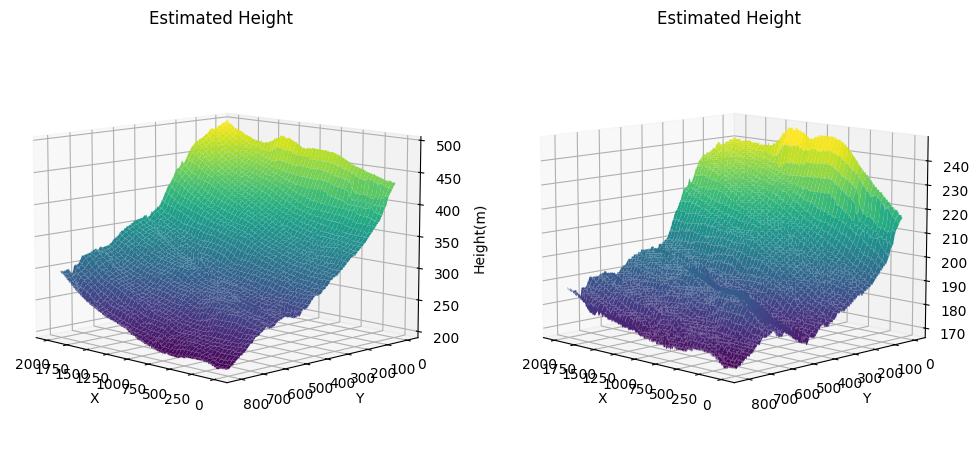
\includegraphics[width=0.9\textwidth]{t1/output3d_1_2.png}
		\caption{最佳高程恢复色度图}
		\label{fig:best_height}
	\end{figure}
	
	最终我们求得的4个顶点的高程值(单位:m,精确到1m)分别为(代码见附录7.9):\par

	\begin{figure}[H]
		\centering
		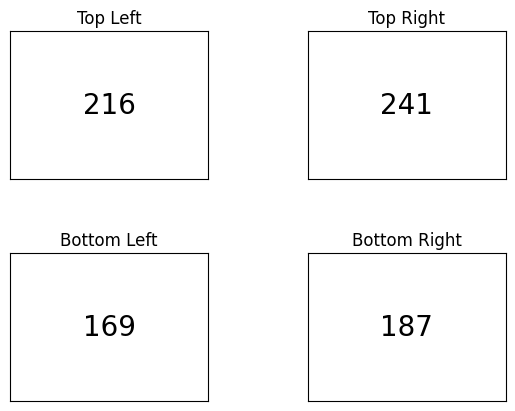
\includegraphics[width=0.5\textwidth]{t1/output_1_1.png}
		\label{fig:4corner}
	\end{figure}

	\subsubsection{结果的验证与分析}

	\paragraph{方差分析和梯度分析}
	使用方差分析和梯度分析可以得到,使用2和5数据解缠、融合后的图像的平滑度均为最佳,如图7所示(红色为融合图像,两种分析方法下的值均最低,说明高程恢复效果很好,代码见附录7.10):\par

	\begin{figure}[H]
		\centering
		\begin{minipage}[b]{0.4\textwidth}
			\centering
			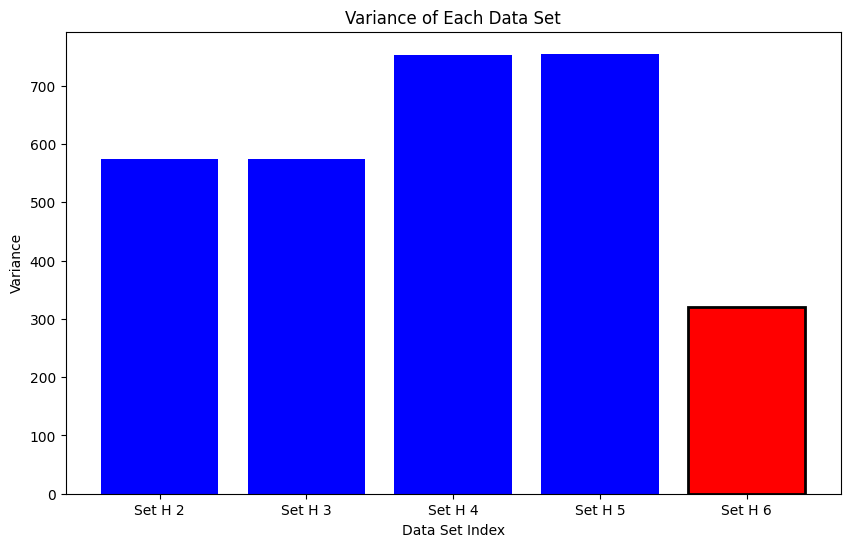
\includegraphics[width=\linewidth]{t1/best_test_1.png}
		\end{minipage}
		\hspace{0.05\textwidth}
		\begin{minipage}[b]{0.4\textwidth}
			\centering
			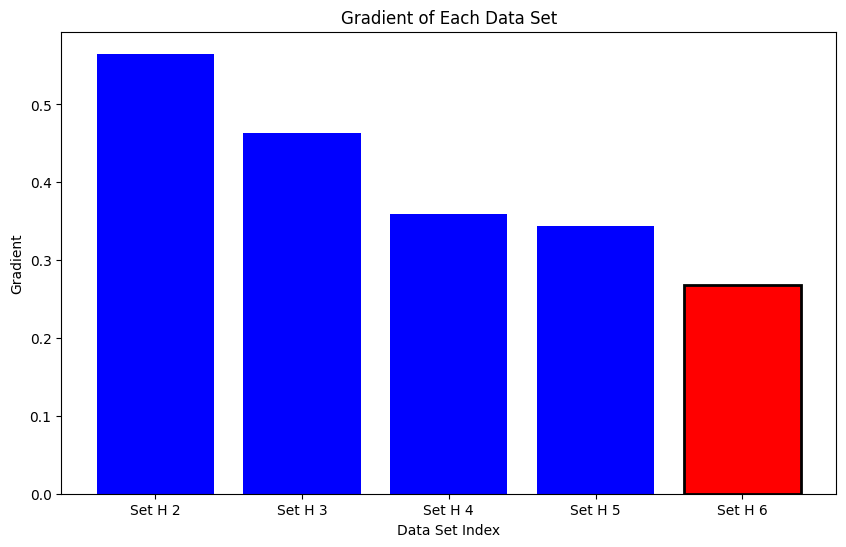
\includegraphics[width=\linewidth]{t1/best_test_2.png}
		\end{minipage}
		
		\caption{方差分析和梯度分析结果显示均为最佳}
		\label{fig:best_height_test}
	\end{figure}

	\paragraph{python内置的unwrap()函数}
	python的numpy模版库中内置一个用于相位解缠和相位折叠恢复的函数unwrap(),我们采用该函数对原数据进行解缠后得到的结果与相位展开法得到的结果吻合得很好:\par

	\begin{figure}[H]
		\centering
		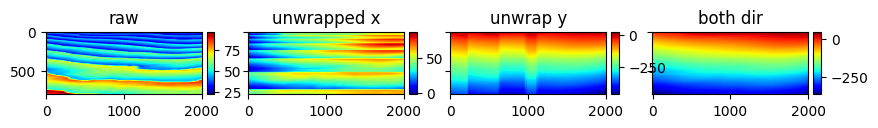
\includegraphics[width=1\textwidth]{t1/inside_unwrap_1.png}
		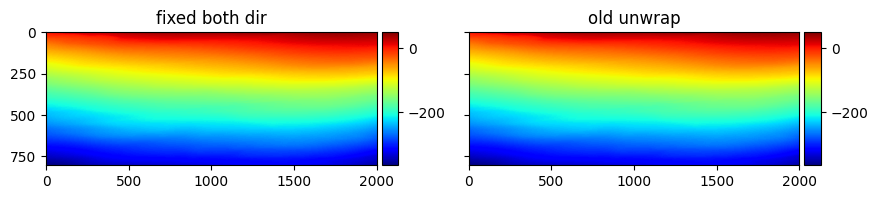
\includegraphics[width=1\textwidth]{t1/inside_unwrap_2.png}
		\caption{unwrap()函数与相位展开法的比较}
		\label{fig:inside_unwrap}
	\end{figure}

	\paragraph{LSTM自动编码器}
	由于可以用光的双缝干涉原理解释一种相位纠缠发生的原因,因此我们人为添加了干涉纹样用于验证该模型的普适性。我们引入了高斯噪声模型(代码见附录7.5):\par
	\begin{equation}
		\phi(x, y) = m_1 x + m_2 y + C + \sum_{n=1}^{N} A_n \exp \Bigg[ - \bigg( \frac{(x - \mu_x)^2}{2\sigma_x^2} + \frac{(y - \mu_y)^2}{2\sigma_y^2} \bigg) \Bigg] \; ; \; \forall (x, y) \in [-128, 127)^2
	\end{equation}
	生成噪声,但在解缠、恢复的过程中出现了个别相位错位的情况(如图9所示),因此需要考虑引入机器学习\footnote{图8中,对于人为生成的高斯噪声(右)的解缠,相位扩展法(左)出现了个别相位错位的现象,而LSTM自动编码器相位解缠的结果(中)非常好。}的方法进行验证和对比(代码见附录7.6)。\par

	\begin{figure}[H]
		\centering
		\begin{minipage}[b]{0.31\textwidth}
			\centering
			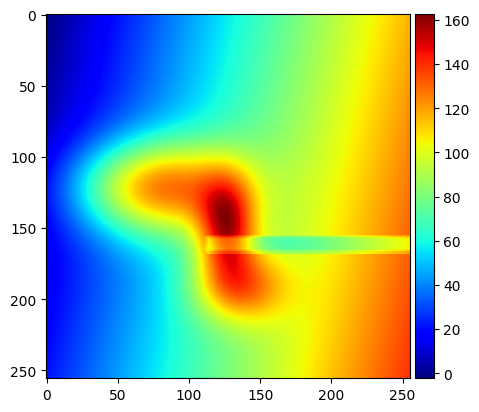
\includegraphics[width=\linewidth]{t1/unwrap_gauss.png}
		\end{minipage}
		\hspace{0.05\textwidth}
		\begin{minipage}[b]{0.6\textwidth}
			\centering
			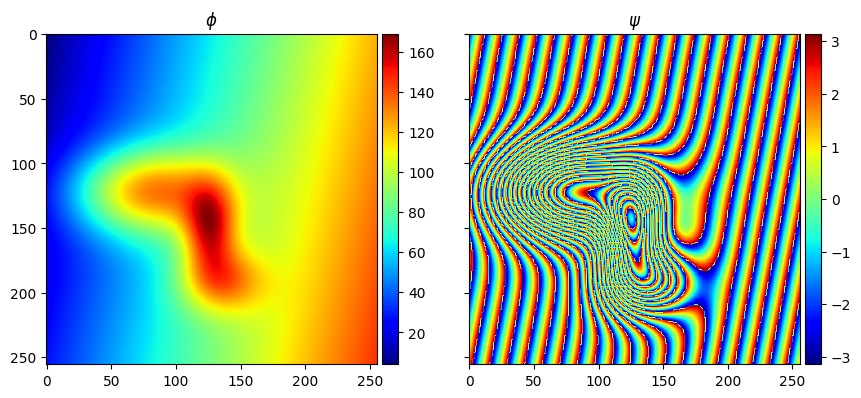
\includegraphics[width=\linewidth]{t1/lstm_gauss.png}
		\end{minipage}
		
		\caption{高斯噪声解缠及高程恢复对比图}
		\label{fig:shortcoming}
	\end{figure}

	
	\subsection{问题二模型的建立与求解}

	问题二的讨论紧承问题一第2小问的思路。从主观分析的角度考虑,参与拟合的数组组数越多,拟合的效果应该越好。考虑所有可能的组合情况,总方案数应为$ \binom{5}{1} + \binom{5}{2} + \binom{5}{3} + \binom{5}{4} + \binom{5}{5} = 31 $(种),在舍弃第一组数据后,总情况数更是降低到了$ \binom{4}{1} + \binom{4}{2} + \binom{4}{3} + \binom{4}{4} = 15 $(种),因此进行可以进行完全遍历,并根据评价指标进行筛选。
	
	目标规划函数示例:
	
	\begin{equation}
		\begin{aligned}
			& \max \quad E_k=\frac{S_k \cdot Y_{i, y}-Z_k \cdot X_{i, y}}{\gamma} \\
			& \text { s.t. }\left\{\begin{array}{l}
				Z_k=\frac{Y_{i, y} \cdot \beta_k}{1-\alpha_k} \\
				S_k=X_{2, y}\left(1+V_k\right)\left(1+\beta_k\right) \\
				\beta_k \in\{1, c\} \\
				c>1 \\
 
			\end{array}\right.
		\end{aligned}
	\end{equation}
	
	\subsection{问题三模型的建立与求解}

	误差的来源有系统误差和随机误差两个部分,二者的产生原因有所不同。系统误差...;随机误差...\par
	下面对这两部分误差的具体表现和影响做出分析:\par
	
	\subsubsection{系统误差}

	\paragraph{相位跳变的检测错误}
	相位展开法中的相位跳变检测是基于当前像素与其相邻像素之间的差值来确定的。如果相位变化不是由真实的相位跳变引起的,而是由于诸如噪声或其他因素引起的,则可能会错误地检测到相位跳变,从而导致展开误差。\par

	\paragraph{相位图的像素密度不足}
	原相位图的分辨率为$ 805 \times 2001 $,这在地形变化连续,起伏程度不大的条件下已经足够。但对于如城市、山地这类地形复杂多变或断崖、峡谷这类存在地形突变的区域,采样精度可能不足,从而导致误差。\par
	以断崖中存在的相位突变为例,在低像素密度相位图中,相邻原数据两相位之间的确应该存在脱离$ [-\pi,\pi] $范围以外的相位差。但本模型的成立是基于充足像素密度下的连续性原理的,因此公式(3b)、(4b)、(5b)、(6c)--(6d)无法适用于这类问题的相位恢复,这是局部误差产生的一个重要原因。\par

	\paragraph{相位展开的累积误差}
	本方法采用了累积的方式来展开相位,每个像素的相位都依赖于其周围像素的相位变化。如果在相位解缠的过程中某处出现了局部误差,这个误差会在展开过程中累积,从而影响最终的展开结果。\par

	\paragraph{边界效应}
	边界像素受周围像素的影响程度很小,且在本模型的递推、迭代的思想下,中间相位的准确性很大程度上取决于边缘相位的准确性(因为这些相位是递推的起点)。所以在处理边界像素时,由于没有足够的相邻像素,从而无法保证其准确性,其中可能存在的误差和错误进一步导致了中间相位的解缠时的误差和错误。\par

	\subsubsection{随机误差}

	\paragraph{}




	
	计算公式模版:
	\begin{equation}
		r=\frac{\sum_{i=1}^n\left(X_i-\bar{X}\right)\left(Y_i-\bar{Y}\right)}{\sqrt{\sum_{i=1}^n\left(X_i-\bar{X}\right)^2} \sqrt{\sum_{i=1}^n\left(Y_i-\bar{Y}\right)^2}}
	\end{equation}
	
	相关系数矩阵模版:
	
	\begin{gather*}
		\begin{bmatrix}
			Variable & a & b & c & d & e & f \\
			a & 1 & 1 & 1 & 1 & 1 & 1 \\
			b & 1 & 1 & 1 & 1 & 1 & 1 \\
			c & 1 & 1 & 1 & 1 & 1 & 1 \\
			d & 1 & 1 & 1 & 1 & 1 & 1 \\
			e & 1 & 1 & 1 & 1 & 1 & 1 \\
			f & 1 & 1 & 1 & 1 & 1 & 1 \\
		\end{bmatrix}
	\end{gather*}
	
	%Part Six
	\section{模型的评价、改进与推广}
	\subsection{模型优点}
	\begin{enumerate}
		\item 本模型深刻理解、应用了雷达波的干涉原理与双缝干涉同根同源的理论基础,对物理规律进行了充分应用,同时采用了其他成熟的方法进行印证,健全可靠。
		\item 本论文给出了大量额外参考图像和计算数据,条分缕析,推理严谨,深入浅出,结果准确。
		\item 本模型的预测准确率高,具有很强的应用价值,可以直接应用于InSAR高程恢复及相关领域。
	\end{enumerate}
	
	\subsection{模型缺点与改进方向}
	\begin{enumerate}
		\item 出于简化计算的考虑,我们在模型设计之初舍弃了第1组相干性较差的数据,但在实际情形中可以预知,这组数据中仍然含有关于正确高程的信息,所以简单的舍弃必然导致额外误差的产生。因此,未来可以考虑如何对像第1组这样包含信息量较少的数据进行充分利用,并将对此类数据的处理方法添加进模型之中。
		\item 
		\item 
	\end{enumerate}
	
	\clearpage

	%Part Seven
	\section{参考文献}
	\vspace{-2em} % 减小上面的间距
	\begin{thebibliography}{9}  
		\bibitem{ref1} 许才军,王华. InSAR相位解缠算法比较及误差分析[J]. 武汉大学学报(信息科学版),2004,29(1):67-71. DOI:10.3969/j.issn.1671-8860.2004.01.015.
		\bibitem{ref2} 邓晓龙. InSAR相位解缠算法的研究[D]. 黑龙江:哈尔滨工业大学,2013. DOI:10.7666/d.D420604.
		\bibitem{ref3} 蒲黎明. 基于深度学习的InSAR数据处理技术研究[D]. 四川:电子科技大学,2022.
		\bibitem{ref4} 黄蓉. InSAR相位解缠算法比较研究[D]. 陕西:长安大学,2012. DOI:10.7666/d.D234691.
		\bibitem{ref5} 刘伟科. InSAR相位解缠非线性最小二乘方法研究[D]. 山东:山东科技大学,2013. DOI:10.7666/d.Y2676909.
		\bibitem{ref6} 张利恒. 喀斯特地貌SAR影像配准方法研究[D]. 广西:桂林理工大学,2013. DOI:10.7666/d.D388608.
		\bibitem{ref7} 刘国林,张连蓬,江涛. 相位解缠中的一致性与非一致性分析[J]. 中国图象图形学报(A辑),2003,8(z1):188-190. DOI:10.3969/j.issn.1006-8961.2003.z1.042.
		\bibitem{ref8} 薛海伟,冯大政. 一种快速的InSAR图像精配准方法[J]. 西安电子科技大学学报(自然科学版),2016,43(3):172-178. DOI:10.3969/j.issn.1001-2400.2016.03.030.
		\bibitem{ref9} 张永俊,黄海风,张永胜,等. InSAR误差建模与误差估计方法[J]. 电子学报,2011,39(6):1225-1230.
		\bibitem{ref10} 张媛媛,于咏梅,王蕾. 基于熵权-变异系数组合权重的金银花质量评价模型构建[J]. 食品安全质量检测学报,2021,12(10):4303-4308.
		\bibitem{ref11} 郭子茵,陈振标,刘敏榕. 基于熵权-TOPSIS法的福建省高校科技创新能力实证研究[J]. 情报探索,2023(5):46-52. DOI:10.3969/j.issn.1005-8095.2023.05.007.
		\bibitem{ref12} 刘国祥,陈强等,InSAR原理与应用,科学出版社,2019.
	\end{thebibliography}
	
	\newpage
	\section*{附录}

	支撑材料的文件列表
	
	\subsection{Raw文件读入与数据预处理}
	\begin{lstlisting}[language=python,columns=fullflexible,frame=shadowbox]
		import math
		import numpy as np
		import pandas as pd
		import matplotlib.pyplot as plt
		from scipy.ndimage import convolve

		df_k = []
		df_theta = []

		for i in range(1,6):
			df_k.append(pd.read_csv(f'./raw_data/kz_{i}.csv', header=None))
			df_theta.append(pd.read_csv(f'./raw_data/Theta_{i}.csv', header=None ))
			
		import re

		for i in range(5):
			print(f'kz_{i+1}.csv shape: {df_k[i].shape}')
			print(f'Theta_{i+1}.csv shape: {df_theta[i].shape}')
			
			for j in range(df_k[i].shape[1]):
				k_j = df_k[i].iloc[0 ,j]
				k_j_str = str(k_j)
				pattern = r"-0\.\d+"
				matches = re.findall(pattern,k_j_str)
				df_k[i].loc[0, j] = float(matches[0])
				
			df_k[i] = pd.DataFrame(np.array(df_k[i]).astype(float))
							
		num_rows = 805
		num_cols = 2001
	\end{lstlisting}

	\subsection{自定义绘图函数}
	\begin{lstlisting}[language=python,columns=fullflexible,frame=shadowbox]
		from mpl_toolkits.mplot3d import Axes3D
		from mpl_toolkits.axes_grid1 import make_axes_locatable

		def draw3D(H):
			N, M = H.shape
			x = np.linspace(1, M, M)
			y = np.linspace(1, N, N)
			x, y = np.meshgrid(x, y)

			fig = plt.figure()
			ax = fig.add_subplot(111, projection='3d')
			ax.plot_surface(x, y, H, cmap='viridis')

			ax.set_title('Estimated Height')
			ax.set_xlabel('X')
			ax.set_ylabel('Y')
			ax.set_zlabel('Height(m)')
			ax.view_init(elev=10, azim=135)

			plt.show()
			
		def plot(*argv, titles=None):
		if len(argv) == 1:
			f, ax = plt.subplots(1, 1, sharey=True, figsize=(5, 5))
			if titles is not None:
			ax.set_title(titles)
			a = ax.imshow(argv[0].squeeze(), cmap='jet')
			divider = make_axes_locatable(ax)
			cax = divider.append_axes("right", size="5%", pad=0.05)
			f.colorbar(a, cax=cax)
			plt.show()
		else:
			f, axes = plt.subplots(1, len(argv), sharey=True, figsize=(10, 10))
			for i in range(len(argv)):
				if titles is not None:
				axes[i].set_title(titles[i])
				a = axes[i].imshow(argv[i].squeeze(), cmap='jet')
				divider = make_axes_locatable(axes[i])
				cax = divider.append_axes("right", size="5%", pad=0.05)
				f.colorbar(a, cax=cax)
			plt.show()
			f.colorbar(a, cax=cax)

		def plot_hist(*argv, titles):
		for i in range(len(argv)):
			hist = np.histogram(argv[i].ravel(), bins=100)
			plt.plot(hist[1][1:], hist[0])
		plt.xlabel("phase values")
		plt.ylabel("frequency")
		plt.title("Histogram Analysis")
		plt.grid()
		if titles is not None:
			plt.legend(titles)
		plt.show()  
	\end{lstlisting}

	\subsection{基于连续性原理的相位展开解缠算法(2维形式)}
	\begin{lstlisting}[language=python,columns=fullflexible,frame=shadowbox]
		def unwrap_phase(theta):
		phi = np.zeros_like(theta)
		phi[0, 0] = theta[0, 0]
		
		for i in range(1, theta.shape[0]):
			delta = theta[i, 0] - theta[i-1, 0]
			delta_wrapped = np.mod(delta + np.pi, 2 * np.pi) - np.pi
			phi[i, 0] = phi[i-1, 0] + delta_wrapped

		for j in range(1, theta.shape[1]):
			delta = theta[0, j] - theta[0, j-1]
			delta_wrapped = np.mod(delta + np.pi, 2 * np.pi) - np.pi
			phi[0, j] = phi[0, j-1] + delta_wrapped

		for i in range(1, theta.shape[0]):
			for j in range(1, theta.shape[1]):
				delta_row = theta[i, j] - theta[i-1, j]
				delta_col = theta[i, j] - theta[i, j-1]
				delta_row_wrapped = np.mod(delta_row + np.pi, 2 * np.pi) - np.pi
				delta_col_wrapped = np.mod(delta_col + np.pi, 2 * np.pi) - np.pi
				phi[i, j] = phi[i-1, j] + delta_row_wrapped
				phi[i, j] = phi[i, j-1] + delta_col_wrapped
				
		return phi	
	\end{lstlisting}

	\subsection{高程还原算法}
	\begin{lstlisting}[language=python,columns=fullflexible,frame=shadowbox]
		h = np.zeros((num_rows, num_cols))

		for i in range(1,5):
			step = (i+1) * 100
			phi = unwrap_phase(np.array(df_theta[i]))
			h = -1 * phi / df_k[i]
			while np.min(h) < 150 or np.max(h) > 300:
				step += 1
				phi += 2 * np.pi
				h = -1 * phi / df_k[i]
				if np.min(h) >= 150 and np.max(h) <= 300:
					plot(df_theta[i], phi, h, titles=["raw $\Theta$", "new $\phi$", f"{step}"])		
	\end{lstlisting}

	\subsection{自主模拟高斯噪声与解缠}
	\begin{lstlisting}[language=python,columns=fullflexible,frame=shadowbox]
		from mpl_toolkits.axes_grid1 import make_axes_locatable

		def simulate(size, m_1, m_2, C, A, mu_x, mu_y, sigma_x, sigma_y):
			x = np.arange(0, size[0], 1)
			y = np.arange(0, size[0], 1)
			xx, yy = np.meshgrid(x, y, sparse=True)
			I = np.zeros(size)
	
			for i in range(len(sigma_x)):
				a = (xx-mu_x[i])**2/(2*sigma_x[i]**2) + (yy-mu_y[i])**2/(2*sigma_y[i]**2)
				I += A[i]*np.exp(-a)
			I = m_1*xx + m_2*yy + C + 0.1*I
			return I
		
		def wrap(phi):
			return np.angle(np.exp(1j*phi))
		
		def rescale(im, range):
			im_std = (im - im.min()) / (im.max() - im.min())
			im_scaled = im_std * (range[1] - range[0]) + range[0]
			return im_scaled
		
		def create_random_image(size):
			array_len = np.random.randint(2, 5)
			m = np.random.uniform(0, 0.5, [2])
			C = np.random.randint(1, 10)
			A = np.random.randint(50, 1000, array_len)
			mu_x = np.random.randint(round(size[0] / 4), round(size[1] * 3 / 4), array_len)
			mu_y = np.random.randint(round(size[0] / 4), round(size[1] * 3 / 4), array_len)
			sigma_x = np.random.randint(10, 45, array_len)
			sigma_y = np.random.randint(10, 45, array_len)
			I = simulate(size, m[0], m[1], C, A, mu_x, mu_y, sigma_x, sigma_y)
			return I
			
		## example
		size = (256, 256)	
		I = create_random_image(size)
		I_wrap = wrap(I)
		plot(I, I_wrap, titles=["$\phi$", "$\psi$"])
		phi = unwrap_phase(I_wrap)

		plot(phi)  		
	\end{lstlisting}

	\subsection{LSTM自动编码器}
	\begin{lstlisting}[language=python,columns=fullflexible,frame=shadowbox]
		import numpy as np
		import h5py
		import os
		import matplotlib as mpl
		mpl.style.use('default')
		import matplotlib.pyplot as plt
		from mpl_toolkits.axes_grid1 import make_axes_locatable
		
		from keras.layers import Activation, BatchNormalization, Conv2D, UpSampling2D, Conv2DTranspose, concatenate
		from keras.layers import MaxPooling2D, Dropout, Input, AveragePooling2D, Reshape, Permute, UpSampling2D
		from keras.layers import SimpleRNN, Bidirectional, LSTM
		from keras.layers import Lambda
		from keras.losses import sparse_categorical_crossentropy
		import tensorflow as tf
		from keras.optimizers import *
		import keras.backend as K
		import keras
		from keras.callbacks import ModelCheckpoint, EarlyStopping
		K.set_image_data_format('channels_last')

		def get_joint_conv_sqd_lstm_net():
			## input to the network
			input = Input((256, 256, 1))
		
			## encoder network
			c1 = Conv2D(filters=16, kernel_size=(3,3), kernel_initializer='he_normal', padding='same')(input)
			c1 = BatchNormalization()(c1)
			c1 = Activation('relu')(c1)
			p1 = AveragePooling2D()(c1)
		
			c2 = Conv2D(filters=32, kernel_size=(3,3), kernel_initializer='he_normal', padding='same')(p1)
			c2 = BatchNormalization()(c2)
			c2 = Activation('relu')(c2)
			p2 = AveragePooling2D()(c2)
		
			c3 = Conv2D(filters=64, kernel_size=(3,3), kernel_initializer='he_normal', padding='same')(p2)
			c3 = BatchNormalization()(c3)
			c3 = Activation('relu')(c3)
			p3 = AveragePooling2D()(c3)
		
			c4 = Conv2D(filters=128, kernel_size=(3, 3), kernel_initializer='he_normal', padding='same')(p3)
			c4 = BatchNormalization()(c4)
			c4 = Activation('relu')(c4)
			p4 = AveragePooling2D()(c4)
		
			# SQD-LSTM Block
			x_hor_1 = Reshape((16 * 16, 128))(p4)
			x_ver_1 = Reshape((16 * 16, 128))(Permute((2, 1, 3))(p4))
		
			h_hor_1 = Bidirectional(LSTM(units=32, activation='tanh', return_sequences=True, go_backwards=False))(x_hor_1)
			h_ver_1 = Bidirectional(LSTM(units=32, activation='tanh', return_sequences=True, go_backwards=False))(x_ver_1)
		
			H_hor_1 = Reshape((16, 16, 64))(h_hor_1)
			H_ver_1 = Permute((2, 1, 3))(Reshape((16, 16, 64))(h_ver_1))
		
			c_hor_1 = Conv2D(filters=64, kernel_size=(3, 3),
							kernel_initializer='he_normal', padding='same')(H_hor_1)
			c_ver_1 = Conv2D(filters=64, kernel_size=(3, 3),
							kernel_initializer='he_normal', padding='same')(H_ver_1)
		
			H = concatenate([c_hor_1, c_ver_1])
		
			# decoder Network
			u5 = Conv2DTranspose(128, (3, 3), strides=(2, 2), padding='same')(H)
			u5 = concatenate([u5, c4])
			c5 = Conv2D(filters=128, kernel_size=(3,3), kernel_initializer='he_normal', padding='same')(u5)
			c5 = BatchNormalization()(c5)
			c5 = Activation('relu')(c5)
		
			u6 = Conv2DTranspose(64, (3, 3), strides=(2, 2), padding='same')(c5)
			u6 = concatenate([u6, c3])
			c6 = Conv2D(filters=64, kernel_size=(3,3), kernel_initializer='he_normal', padding='same')(u6)
			c6 = BatchNormalization()(c6)
			c6 = Activation('relu')(c6)
		
			u7 = Conv2DTranspose(32, (3, 3), strides=(2, 2), padding='same')(c6)
			u7 = concatenate([u7, c2])
			c7 = Conv2D(filters=32, kernel_size=(3,3), kernel_initializer='he_normal', padding='same')(u7)
			c7 = BatchNormalization()(c7)
			c7 = Activation('relu')(c7)
		
			u8 = Conv2DTranspose(16, (3, 3), strides=(2, 2), padding='same')(c7)
			u8 = concatenate([u8, c1])
			c8 = Conv2D(filters=32, kernel_size=(3,3), kernel_initializer='he_normal', padding='same')(u8)
			c8 = BatchNormalization()(c8)
			c8 = Activation('relu')(c8)
		
			## output layer
			output = Conv2D(filters=1, kernel_size=(1, 1), padding='same', name='out1')(c8)
			output = Activation('linear')(output)
		
			model = Model(inputs=[input], outputs=[output])
			return model

		Model = lambda df_theta: [unwrap_phase(np.array(df_theta[i])) for i in range(5)]
		Model = get_joint_conv_sqd_lstm_net()
		model_path = './model/LSTM_model.h5'
		Model.load_weights(model_path)
	\end{lstlisting}

	\subsection{基于连续性原理的相位展开解缠算法(3维形式)}
	\begin{lstlisting}[language=python,columns=fullflexible,frame=shadowbox]
		def unwrap_3D_phase(theta):
			phi = np.zeros_like(theta)
			phi[0, 0, 0] = theta[0, 0, 0]
				
			for k in range(0, theta.shape[2]):
				for i in range(1, theta.shape[0]):
					delta = theta[i, 0, k] - theta[i-1, 0, k]
					delta_wrapped = np.mod(delta + np.pi, 2 * np.pi) - np.pi
					phi[i, 0, k] = phi[i-1, 0, k] + delta_wrapped
				
				for j in range(1, theta.shape[1]):
					delta = theta[0, j, k] - theta[0, j-1, k]
					delta_wrapped = np.mod(delta + np.pi, 2 * np.pi) - np.pi
					phi[0, j, k] = phi[0, j-1, k] + delta_wrapped
					
				for i in range(1, theta.shape[0]):
					for j in range(1, theta.shape[1]):
						delta_row = theta[i, j, k] - theta[i-1, j, k]
						delta_col = theta[i, j, k] - theta[i, j-1, k]
						delta_row_wrapped = np.mod(delta_row + np.pi, 2 * np.pi) - np.pi
						delta_col_wrapped = np.mod(delta_col + np.pi, 2 * np.pi) - np.pi
						phi[i, j, k] = phi[i-1, j, k] + delta_row_wrapped
						phi[i, j, k] = phi[i, j-1, k] + delta_col_wrapped
					
			depth = lambda theta, phi: np.array([[[phi[i-1, j, k] + (np.mod(theta[i, j, k] - theta[i-1, j, k] + np.pi, 2 * np.pi) - np.pi) if i > 0 else phi[i, j, k],
												phi[i, j-1, k] + (np.mod(theta[i, j, k] - theta[i, j-1, k] + np.pi, 2 * np.pi) - np.pi) if j > 0 else phi[i, j, k],
												phi[i, j, k-1] + (np.mod(theta[i, j, k] - theta[i, j, k-1] + np.pi, 2 * np.pi) - np.pi) if k > 0 else phi[i, j, k]]
												for j in range(theta.shape[1])]])
			
			return phi
	\end{lstlisting}

	\subsection{2组数据的相位融合算法}
	\begin{lstlisting}[language=python,columns=fullflexible,frame=shadowbox]
		combine_2_5 = np.zeros((num_rows, num_cols, 2))

		for i in range(num_rows):
			for j in range(num_cols):
				combine_2_5[i][j][0] = Y_pred[1][i][j]
				combine_2_5[i][j][1] = Y_pred[4][i][j]
		
		weight = np.zeros((2,1))
		weight1 = s[1] / (s[1] + s[4])
		weight2 = s[4] / (s[1] + s[4])
		weight[0][0] = weight1
		weight[1][0] = weight2
		
		combine_2_5 = unwrap_3D_phase(combine_2_5)
		combine = np.zeros((num_rows, num_cols))
		
		tmp = np.zeros((num_rows, num_cols))
		
		combine = combine_2_5 @ weight		
		combine = combine.ravel().reshape((num_rows,num_cols))
	
		plot(combine, titles="combined $\phi$")
		
		plot((-1 * combine / df_k[1]), (-1 * combine / df_k[4]), titles=["Height 0", "Height 1"])
		
		H = -1 * combine / df_k[1]		
		N, M = H.shape
		x = np.linspace(1, M, M)
		y = np.linspace(1, N, N)
		x, y = np.meshgrid(x, y)
		fig = plt.figure(figsize=(12, 6))
		ax1 = fig.add_subplot(121, projection='3d')
		ax1.plot_surface(x, y, H, cmap='viridis')
		ax1.set_title('Estimated Height')
		ax1.set_xlabel('X')
		ax1.set_ylabel('Y')
		ax1.set_zlabel('Height(m)')
		ax1.view_init(elev=10, azim=135)
		
		H = -1 * combine / df_k[4]	
		N, M = H.shape
		x = np.linspace(1, M, M)
		y = np.linspace(1, N, N)
		x, y = np.meshgrid(x, y)
		ax2 = fig.add_subplot(122, projection='3d')
		ax2.plot_surface(x, y, H, cmap='viridis')
		ax2.set_title('Estimated Height')
		ax2.set_xlabel('X')
		ax2.set_ylabel('Y')
		ax2.set_zlabel('Height(m)')
		ax2.view_init(elev=10, azim=135)
		
		plt.show()		
	\end{lstlisting}

	\subsection{四角高程值计算}
	\begin{lstlisting}[language=python,columns=fullflexible,frame=shadowbox]
		print(H.shape)

		final = np.array(H)

		top_left = round(final[0, 0])
		top_right = round(final[0, num_cols-1])
		bottom_left = round(final[num_rows-1, 0])
		bottom_right = round(final[num_rows-1, num_cols-1])
		
		fig, axs = plt.subplots(2, 2)
		
		# 设置四个顶点的值
		axs[0, 0].text(0.5, 0.5, str(top_left), ha='center', va='center', size=20)
		axs[0, 0].set_title('Top Left')
		axs[0, 1].text(0.5, 0.5, str(top_right), ha='center', va='center', size=20)
		axs[0, 1].set_title('Top Right')
		axs[1, 0].text(0.5, 0.5, str(bottom_left), ha='center', va='center', size=20)
		axs[1, 0].set_title('Bottom Left')
		axs[1, 1].text(0.5, 0.5, str(bottom_right), ha='center', va='center', size=20)
		axs[1, 1].set_title('Bottom Right')
		
		for ax in axs.flat:
			ax.set(xticks=[], yticks=[])
		
		plt.subplots_adjust(hspace=0.5, wspace=0.5)	
		plt.show()		
	\end{lstlisting}

	\subsection{方差分析和梯度平均}
	\begin{lstlisting}[language=python,columns=fullflexible,frame=shadowbox]
		## 方差分析
		vars = []
		vars_for_dis = []
		hs = []
		
		h = np.zeros((num_rows, num_cols))
		for i in range(1,5):
			phi = unwrap_phase(Y_pred[i])
			h = -1 * phi / df_k[i]
			while np.min(h) < 150 or np.max(h) > 300:
				phi += 2 * np.pi
				h = -1 * phi / df_k[i]
				if np.min(h) >= 150 and np.max(h) <= 300:
					hs.append(h)
					vars.append(np.array(h).flatten())
			
					
		for i in range(1,5):
			vars_for_dis.append(np.var(vars[i-1], ddof=1))
		
		vars_for_dis.append(np.var(final.flatten(), ddof=1))
		hs.append(final)
			
		## 梯度平均
		hs_for_dis = []

		for i in range(1, 6):   
			gradient_x, gradient_y = np.gradient(np.array(hs[i-1]))
			gradient_magnitude = np.sqrt(gradient_x**2 + gradient_y**2)
			# 计算梯度的平均值作为光滑程度的指标
			smoothness_gradient = np.mean(gradient_magnitude)
			hs_for_dis.append(smoothness_gradient)
		
		## 共用的可视化代码
		# 创建直方图
		plt.figure(figsize=(10, 6))
		bars = plt.bar(range(len(hs_for_dis)), hs_for_dis, color='b')
		
		# 高亮最后一个数据
		bars[-1].set_color('r')
		bars[-1].set_edgecolor('black')
		bars[-1].set_linewidth(2)
		
		# 添加标签和标题
		plt.xlabel('Data Set Index')
		plt.ylabel('Gradient')
		plt.title('Gradient of Each Data Set')
		plt.xticks(range(len(hs_for_dis)), [f'Set H {i+2}' for i in range(len(hs_for_dis))])
		
		plt.show() 				
	\end{lstlisting}

	\subsection{}
	\begin{lstlisting}[language=python,columns=fullflexible,frame=shadowbox]

	\end{lstlisting}

	\subsection{}
	\begin{lstlisting}[language=python,columns=fullflexible,frame=shadowbox]

	\end{lstlisting}
	
\end{document}